% HFUT_Courge_Project
\documentclass[UTF8]{ctexart}
\usepackage{fancyhdr}
\usepackage{graphicx}
\usepackage{titlesec}
\usepackage{titletoc}
\usepackage{listings}
\usepackage{appendix}
\usepackage{bm, amsmath,amsfonts}
\usepackage{multirow}
\usepackage[a4paper,left=3.4cm,right=3cm,top=1.65cm,bottom=2.54cm]{geometry}
\renewcommand{\contentsname}{\zihao{3} 目\quad 录}
\renewcommand{\abstractname}{\zihao{3} 摘\quad 要}
%页眉页脚设置
\pagestyle{fancy}
\fancyhf{}
\cfoot{\thepage}
%\rhead{\kaishu~XX课程设计~}

%目录页设置
\titlecontents{section}[0em]{\zihao{4}\bf }{\thecontentslabel\ }{}
{\hspace{.5em}\titlerule*[4pt]{$\cdot$}\contentspage}
\titlecontents{subsection}[2em]{\vspace{0.1\baselineskip}\zihao{-4}}{\thecontentslabel\ }{}
{\hspace{.5em}\titlerule*[4pt]{$\cdot$}\contentspage}
\titlecontents{subsubsection}[4em]{\vspace{0.1\baselineskip}\zihao{-4}}{\thecontentslabel\ }{}
{\hspace{.5em}\titlerule*[4pt]{$\cdot$}\contentspage}
%代码设置
\RequirePackage{listings}
\RequirePackage{xcolor}
\definecolor{dkgreen}{rgb}{0,0.6,0}
\definecolor{gray}{rgb}{0.5,0.5,0.5}
\definecolor{mauve}{rgb}{0.58,0,0.82}
\lstset{
	numbers=left,  
	frame=tb,
	aboveskip=3mm,
	belowskip=3mm,
	showstringspaces=false,
	columns=flexible,
	framerule=1pt,
	rulecolor=\color{gray!35},
	backgroundcolor=\color{gray!5},
	basicstyle={\ttfamily},
	numberstyle=\tiny\color{gray},
	keywordstyle=\color{blue},
	commentstyle=\color{dkgreen},
	stringstyle=\color{mauve},
	breaklines=true,
	breakatwhitespace=true,
	tabsize=3,
}
%------------------------------------------------------------------------
%正文部分
\begin{document}
	\begin{titlepage}
               	
\includegraphics[width=3.0cm,height=3.0cm]{gdut1.jpg}\\

		%\vspace*{1.5cm}
		\centering
		\quad
\includegraphics[width=13cm,height=4cm]{gdut.jpg}\\
		\vspace*{0.5cm}
		{\fontsize{30pt}\baselineskip 现\quad\ 代\quad\ 控\quad\ 制\quad\ 理\quad\ 论\quad\ 基\quad\ 础}\\

		 \vskip 2.0cm
		 \fontsize{19pt}\baselineskip
		 \makebox[30mm]{题目名称}
		 \underline{\makebox[75mm][c]{  大作业}}\\%在这里修改成自己的题目
		 \vskip 0.9cm
		 \makebox[30mm]{学生姓名}
		 \underline{\makebox[75mm][c]{xxx}}\\
		 \vskip 0.9cm
		 \makebox[30mm]{学\qquad\qquad 号}
		 \underline{\makebox[75mm][c]{ \LARGE12345678}}\\
		 \vskip 0.9cm
		 \makebox[30mm]{专业班级}
		 \underline{\makebox[75mm][c]{xxxxxx}}\\
		 \vskip 0.9cm
		  \makebox[30mm]{指导教师}
		 \underline{\makebox[75mm][c]{ xxx}}\\
		 \vskip 2cm
		 \LARGE \textbf{\number \year }~年~\textbf{\number\month}~月~\textbf{\number\day}~日		 
	\end{titlepage}



\tableofcontents\thispagestyle{empty}
\newpage
\setcounter{page}{1}
\section{基于状态空间表达式的控制器设计方法 }
\subsection{ 模型的建立}
\par 对于SISO LTI系统,状态空间形式如下:
\begin{equation}
   \left  \{\begin{aligned}
      \dot x=Ax+Bu    \\
      y=Cx+D     \\
        \end{aligned}\\
    \right.
 \end{equation}
 
\par 
其中$ \mathbf {X} $是表示系统状态变量的n乘1矢量,$ U $是表示输入的标量,$ Y $是表示输出的标量。矩阵$ A $(n乘n),$ B $(n乘1)和$ C $(1乘n)确定状态变量与输入和输出之间的关系。注意,有n个一阶微分方程。状态空间表示也可用于具有多输入和多输出(MIMO)的系统,但我们将主要用单输入单输出(SISO)系统。
\par  为了介绍状态空间控制设计方法,我们将以磁悬浮球为例。通过线圈的电流引起磁力,该磁力可以平衡重力并使球(由磁性材料制成)悬浮在半空中,如下图:

\par \begin{figure}[h]   
 \center{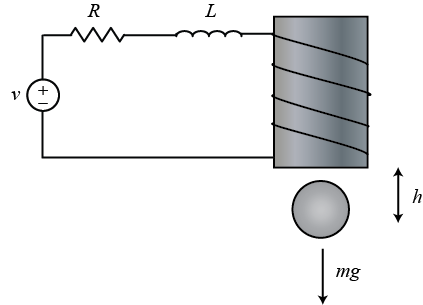
\includegraphics[width=8cm]  {fig/1.png}} 
  \caption{\label{1} 磁悬浮球模型}      
 \end{figure}
 
\par 系统的方程式由下式给出:
\begin{equation}
m\frac {d^{2}h}{dt^{2}}=mg- \frac {Ki^{2}}{h}
\end{equation}

\begin{equation}
V=L\frac {di}{dt}+iR
\end{equation}

\par  $ h $球的垂直位置距离,$ i $是通过电磁铁的电流,$ V $是施加的电压,$ m $是球的质量,$ g $是由重力引起的加速度,$ L $是电感,$ R $是电阻,$ K $是决定电阻的系数施加在球上的磁力。为简单起见,我们将选择值$ m $= 0.05 kg,$ K $= 0.0001,$ L $= 0.01 H,$ R $= 1 Ohm,$ g $= 9.81m/s$^{2}$。只要$ h $=K i$^{2}$/mg(此时$\frac {dh}{dt}$= 0),系统处于平衡状态(球悬浮在半空中)。我们将关于该点的方程线性化$ h $ = 0.01 m(标称电流约为7安培)并获得状态空间方程如下:
\par \begin{equation}
   \left  \{\begin{aligned}
      \dot x=Ax+Bu    \\
      y=Cx+D     \\
        \end{aligned}\\
    \right.
 \end{equation}
\par 其中
\begin{equation}
    x=\begin{bmatrix}
    \triangle h\\
    \triangle \dot h\\
    \triangle i\\
    \end{bmatrix}
\end{equation}
\par 是系统的状态变量集(3x1向量),$ u $是输入电压与其平衡值($ \Delta V $)$ y $的偏差,(输出)是球高度与其平衡位置($ \Delta h $)的偏差。将系统矩阵输入到m文件中。
\par  \begin{lstlisting}[language=matlab,escapeinside=``]
clear all
close all
clc

A = [ 0   1   0;980  0  -2.8;0   0  -100 ];
B = [ 0;0;100 ];
C = [ 1 0 0 ];
\end{lstlisting}

\subsection{ 系统稳定性分析}
\par 首先,分析开环系统(没有任何控制)是否稳定,系统矩阵的特征值$ A $(等于传递函数的极点)决定了稳定性。$ A $矩阵的特征值是特征方程$ \ det(sI  -  A)= 0 $的解 $ s $。
\par  \begin{lstlisting}[language=matlab,escapeinside=``]
poles = eig(A)

poles =
   31.3050
  -31.3050
 -100.0000
\end{lstlisting}
\par 从上面结果可以看出,其中一个极点位于右半平面(即具有正实部),这意味着开环系统不稳定。

\par 当初始条件非零时,此不稳定系统会怎样变化,可以通过Matlab仿真:
\par  \begin{lstlisting}[language=matlab,escapeinside=``]
t = 0:0.01:2;
u = zeros(size(t));
x0 = [0.01 0 0];
sys = ss(A,B,C,0);
[y,t,x] = lsim(sys,u,t,x0);
plot(t,y)
title('Open-Loop Response to Non-Zero Initial Condition')
grid on
\end{lstlisting}
\par 仿真图像如下:
\newpage
\par \begin{figure}[ht]   
 \center{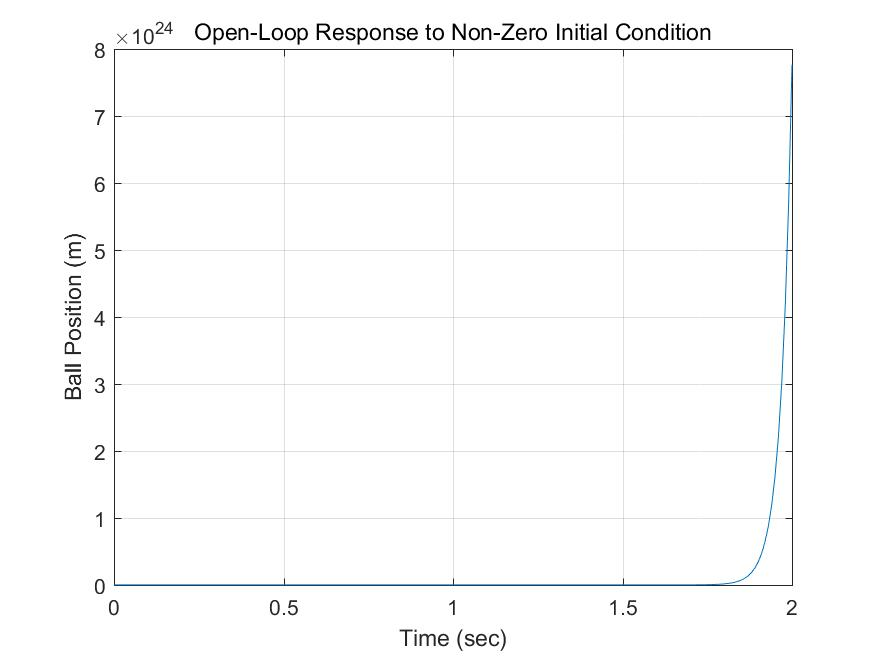
\includegraphics[width=8cm]  {fig/2.jpg}} 
  \caption{\label{1} 初始条件非零系统响应曲线}      
 \end{figure}
\par 从图像可以看出球和电磁铁之间的距离将变为无穷大,可能是球首先击中桌子或地板(也可能超出模型线性化的有效范围)。

\subsection{ 系统的可控性和可观性}
\par 如果总是存在控制输入,则系统是可控的$ u(t)$,该控制输入在有限时间内将系统的任何状态转移到任何其他状态。可以证明,当且仅当其控制矩阵$ \mathcal {C} $具有满秩时(即,如果rank($ \mathcal {C} $)= n,其中n是状态变量的数量),该系统是可控的。可以使用命令rank(ctrb(A,B))或rank(ctrb(sys))在MATLAB中确定LTI模型的可控性矩阵的等级。
\begin{equation}
    C=\begin{bmatrix}
    B & AB & A^{2}B & \ldots & A^{n-1}B\\
    \end{bmatrix}
\end{equation}
\par  系统的所有状态变量可能无法直接测量,例如,如果组件位于不可访问的位置。在这些情况下,有必要仅使用可用的系统输出来估计未知内部状态变量的值。如果初始状态下,$ x(t_0)$,可以确定基于系统输入的知识,$ u(t)$以及系统输出,$ y(t)$,过一些有限的时间间隔$ t_0 <t <t_f $,那么系统是可观的,。对于LTI系统,当且仅当可观矩阵 $\mathcal \emptyset$  具有满秩(即rank($\mathcal \emptyset$)= n,其中n是状态变量的数量)时,系统是可观的。可以使用该命令在MATLAB中确定LTI模型的可观性 rank(obsv(A,C))或rank(obsv(sys))。
\begin{equation}
    \emptyset =\begin{bmatrix}
    C\\CA\\ CA^{2}\\ \ldots \\ CA^{n-1}\\
    \end{bmatrix}
\end{equation}
\par 可控性和可观察性是双重概念。当且仅当系统($ A'$,$ B'$)是可观察的时,系统($ A $,$ B $)是可控的。

\subsection{ 使用极点配置的控制设计}
\par   下面就是使用极点放置方法为该系统设计一个控制器。全状态反馈系统的原理图如下所示。对于这个系统,我们需要一个传感器测量球的位置,另一个测量球的速度,第三个测量电磁铁中的电流。
\newpage
\par \begin{figure}[ht]   
 \center{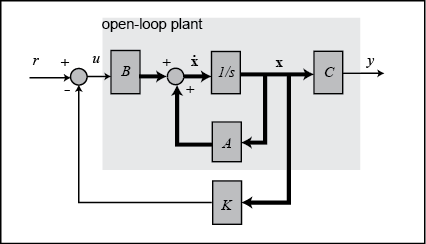
\includegraphics[width=8cm]  {fig/3.png}} 
  \caption{\label{1} 全状态反馈系统的原理图}      
 \end{figure}
\par    为简单起见,假设$ r $= 0.输入如下:
\begin{equation}
u=-Kx
\end{equation}
\par 因此,闭环反馈系统的状态空间方程是
\par \begin{equation}
   \left  \{\begin{aligned}
      \dot x=Ax+B(-Kx)=(A-BK)x    \\
      y=Cx    \\
        \end{aligned}\\
    \right.
 \end{equation}
\par  闭环反馈系统的稳定性和时域性能主要由矩阵($ A-BK $)的特征值的位置确定,其等于闭环极点。由于矩阵$ A $和$ BK $均为3×3,将有3个极的系统。通过选择合适的状态反馈增益矩阵$ K $,我们可以将这些闭环极点放在我们想要的任何地方(因为系统是可控的)。我们可以使用MATLAB函数 来找到状态反馈增益$ K $,它将提供所需的闭环极点。
\par  假设控制器的标准是建立时间$<0.5$秒且过冲$<5%$,那么我们可能会尝试将两个主极点置于-10$\pm$10i( $\zeta$= 0.7$^{\circ}$或45$^{\circ}$,$ \sigma$= 10$>$ 4.6 * 2) 。第三个极点在-50处开始(因此它足够快以至于它对响应没有太大影响):
\par  \begin{lstlisting}[language=matlab,escapeinside=``]
A = [ 0   1   0;980  0  -2.8;0   0  -100 ];
B = [ 0;0;100 ];
C = [ 1 0 0 ];
poles = eig(A)


t = 0:0.01:2;
u = zeros(size(t));
x0 = [0.01 0 0];

p1 = -10 + 10i;
p2 = -10 - 10i;
p3 = -50;
K= place(A,B,[p1 p2 p3]);
sys_cl = ss(A-B*K,B,C,0);
lsim(sys_cl,u,t,x0);
xlabel('Time (sec)')
ylabel('Ball Position (m)')
grid on
\end{lstlisting}
\par \begin{figure}[ht]   
 \center{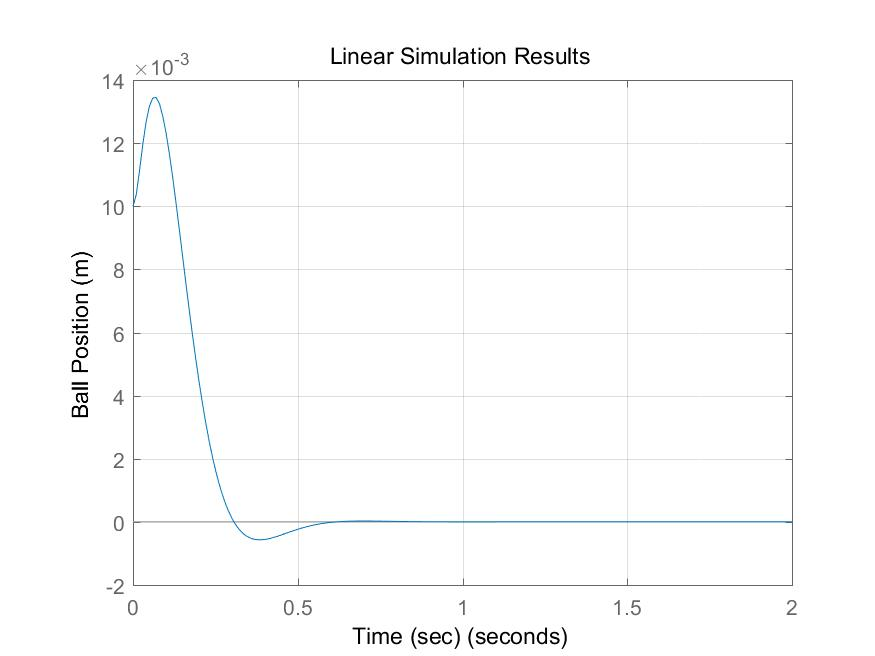
\includegraphics[width=8cm]  {fig/4.jpg}} 
  \caption{\label{1} 闭环极点配置的仿真图像}      
 \end{figure}
\par 从图像可以看到过冲太大。尝试将极点放在左侧以查看瞬态响应是否有所改善。
\par  \begin{lstlisting}[language=matlab,escapeinside=``]
clear all
close all
clc

A = [ 0   1   0;980  0  -2.8;0   0  -100 ];
B = [ 0;0;100 ];
C = [ 1 0 0 ];
poles = eig(A)
p1 = -20 + 20i;
p2 = -20 - 20i;
p3 = -100;

K = place(A,B,[p1 p2 p3]);
sys_cl = ss(A-B*K,B,C,0);
lsim(sys_cl,u,t,x0);
xlabel('Time (sec)')
ylabel('Ball Position (m)')
 grid on
\end{lstlisting}
\newpage
\par \begin{figure}[ht]   
 \center{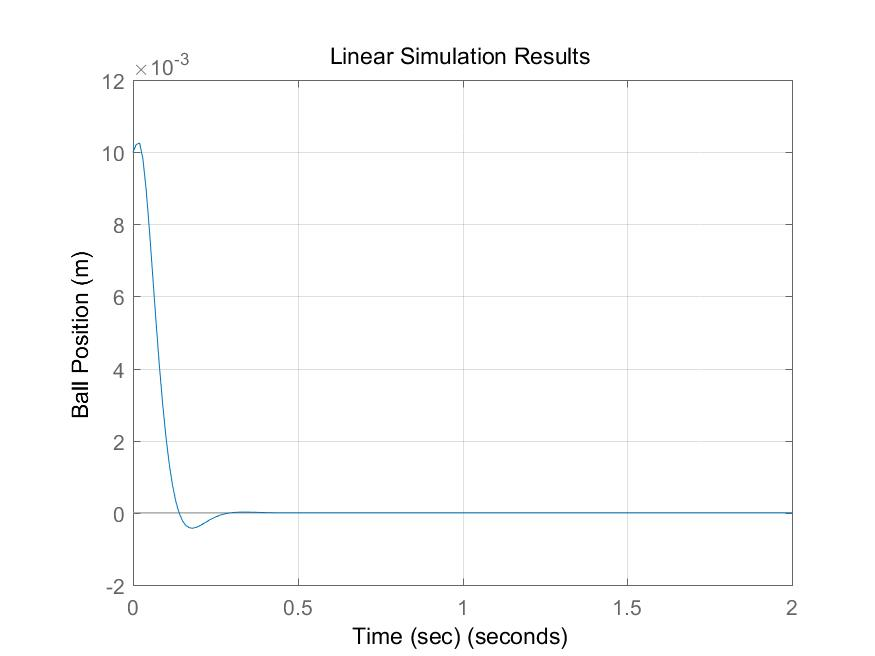
\includegraphics[width=8cm]  {fig/5.jpg}} 
  \caption{\label{1} 闭环极点配置的仿真图像}      
 \end{figure}
\par  这次过冲较小,比较两种情况下所需的控制力($ u $)。通常,将杆子向左移动得越远,需要的控制力就越大。
	
\subsection{实验总结与心得}	
\par  	通过这次大作业,我学会了对物理模型进行转换成数学的状态空间表达式。	通过对系统的控制器的设计,在Matlab下的仿真,加深理解课本的理论知识,同时提高自己的实践技能。
\end{document}